\documentclass{amsart}
\usepackage[utf8]{inputenc}

\title{Desenhos Interessantes}
\author{Geraldo Xexéo}
\date{July 2017}
\usepackage{pgf,tikz}
\usepackage{mathrsfs}
\usetikzlibrary{arrows}
\usetikzlibrary{arrows.meta}
\usetikzlibrary{mindmap} 
\usetikzlibrary{datavisualization}
\usetikzlibrary{datavisualization.formats.functions}
\usetikzlibrary{shapes.misc}
\usetikzlibrary{calc}
\usetikzlibrary{math}
\usetikzlibrary{shapes.symbols}
\usetikzlibrary{shapes.geometric}
\usetikzlibrary{patterns} 
\usetikzlibrary{shadows} 
\usetikzlibrary{automata} % state accepting
\usetikzlibrary{positioning}  % on grid
\usetikzlibrary{topaths}
\usetikzlibrary{intersections}
\usetikzlibrary{decorations} 
\usetikzlibrary{decorations.shapes}
\usetikzlibrary{decorations.pathmorphing}
\usetikzlibrary{decorations.text}
\usepgflibrary{decorations.pathreplacing} 
\usepgflibrary{decorations.markings} 
\usepgflibrary{decorations.footprints} 
\usepgflibrary{decorations.fractals} 
\usetikzlibrary{matrix,arrows} 
\usepackage[all,cmtip]{xy}

\begin{document}

\maketitle

\section{Transparências, Fades, Opacidade}

\tikzfading[name=fade out,
            inner color = transparent!0,
            outer color = transparent!70]

\begin{figure}[h]
\centering
\def\firstcircle{(0,0) circle (1.5cm)}
\def\secondcircle{(0:2cm) circle (1.5cm)}
\begin{tikzpicture}[opacity=0.5]
 \fill [path fading=fade out,
        fading transform={xshift=0.3cm,
        yshift=0.5cm}] \firstcircle;
\end{tikzpicture}
    \caption{Transformando o shading}
\end{figure}

\begin{figure}[h]
\centering
\def\firstcircle{(0,0) circle (1.5cm)}
\def\secondcircle{(0:2cm) circle (1.5cm)}
\begin{tikzpicture}[blend group=multiply]
 \fill [red,path fading=fade out] \firstcircle;
 \fill [blue,path fading=fade out] \secondcircle;
    \draw \firstcircle node[below] {$A$}
          \secondcircle node[below=1.5cm] {$B$};
    \node[anchor=south] at (current bounding box.north) {$A \cup B$};
    
\end{tikzpicture}
    \caption{Multiplicando cores fading}
\end{figure}


\section{Lógica Fuzzy}

Desenhos difíceis, com muitos triângulos, preenchimentos, posicionamentos relativos.

\begin{figure}[h]
\centering
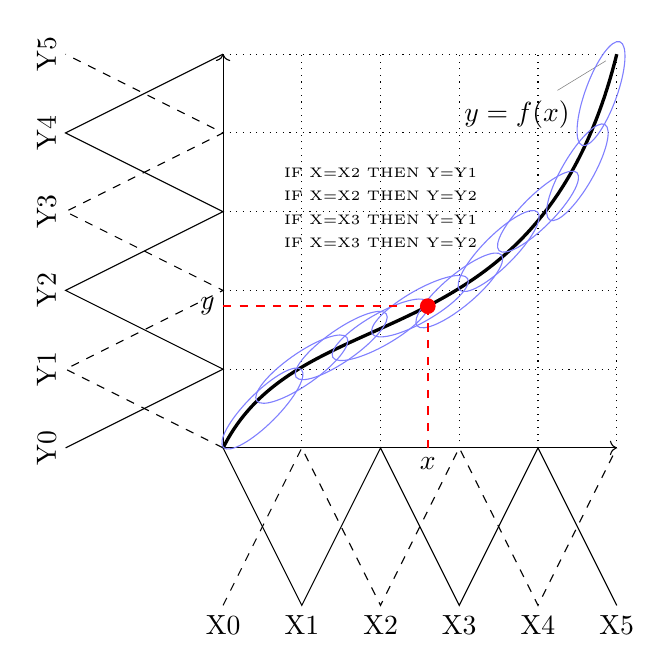
\begin{tikzpicture}

% eixos
\draw[<->] (0,5) -- (0,0) -- (5,0);
\node
at (-.2,1.8) {$y$};
\node[below] at (2.6,0) {$x$};

% triangulos horizontais
\draw (0,0) -- (1,-2) node[below] {X1}-- (2,0) --
        (3,-2) node[below] {X3 }-- (4,0) -- (5,-2) node[below] {X5};
\draw[dashed] (0,-2) node[below] {X0}-- (1,0) -- (2,-2) node[below] {X2} --
        (3,0)-- (4,-2) node[below] {X4} -- (5,0);

% triangulos verticais
\draw (-2,0) node[rotate=90,above] {Y0} -- (0,1) -- (-2,2) node[rotate=90,above] {Y2} --
        (0,3)-- (-2,4) node[rotate=90,above] {Y4} -- (0,5);
\draw[dashed] (0,0) -- (-2,1) node[rotate=90,above] {Y1} -- (0,2) --
        (-2,3) node[rotate=90,above] {Y3} -- (0,4) -- (-2,5) node[rotate=90,above] {Y5};

% retas verticais
\draw[dotted] (1,0) -- (1,5);
\draw[dotted] (2,0) -- (2,5);
\draw[dotted] (3,0) -- (3,5);
\draw[dotted] (4,0) -- (4,5);
\draw[dotted] (5,0) -- (5,5);

% retas horizontais
\draw[dotted] (0,1) -- (5,1);
\draw[dotted] (0,2) -- (5,2);
\draw[dotted] (0,3) -- (5,3);
\draw[dotted] (0,4) -- (5,4);
\draw[dotted] (0,5) -- (5,5);



\draw[very thick] (0,0) coordinate (a1) .. controls  (1,2) and (4,1) .. (5,5) coordinate (a2) node[pin=below left:{$y=f(x)$}] { }  ;

\draw[blue!50,rotate around={45:(0.5,0.5)}] (0.5,0.5) ellipse [x radius=0.7, y radius=0.2];

\draw[blue!50,rotate around={35:(1,1)}] (1,1) ellipse [x radius=0.7, y radius=0.2];

\draw[blue!50,rotate around={35:(1.5,1.3)}] (1.5,1.3) ellipse [x radius=0.7, y radius=0.2];

\draw[blue!50,rotate around={30:(2,1.5)}] (2,1.5) ellipse [x radius=0.7, y radius=0.2];

\draw[blue!50,rotate around={30:(2.5,1.8)}] (2.5,1.8) ellipse [x radius=0.7, y radius=0.2];

\draw[blue!50,rotate around={40:(3,2)}] (3,2) ellipse [x radius=0.7, y radius=0.2];

\draw[blue!50,rotate around={45:(3.5,2.5)}] (3.5,2.5) ellipse [x radius=0.7, y radius=0.2];

\draw[blue!50,rotate around={45:(4,3)}] (4,3) ellipse [x radius=0.7, y radius=0.2];

\draw[blue!50,rotate around={60:(4.5,3.5)}] (4.5,3.5) ellipse [x radius=0.7, y radius=0.2];

\draw[blue!50,rotate around={70:(4.8,4.5)}] (4.8,4.5) ellipse [x radius=0.7, y radius=0.2];

\draw[thick,red,dashed] (2.6,0) -- (2.6,1.8);
\draw[thick,red,dashed] (0,1.8) -- (2.6,1.8);
\fill[red] (2.6,1.8) circle [radius=0.1];

\node[font=\tiny] at (2,3.5) {IF X=X2 THEN Y=Y1};
\node[font=\tiny] at (2,3.2) {IF X=X2 THEN Y=Y2};    
\node[font=\tiny] at (2,2.9) {IF X=X3 THEN Y=Y1};
\node[font=\tiny] at (2,2.6) {IF X=X3 THEN Y=Y2};    

\end{tikzpicture}
\caption{Regras fuzzy funcionam como especificação de pedaços das funções sendo agregadas }
    \label{fig:PDF}
\end{figure}



\begin{figure}[h]
\centering
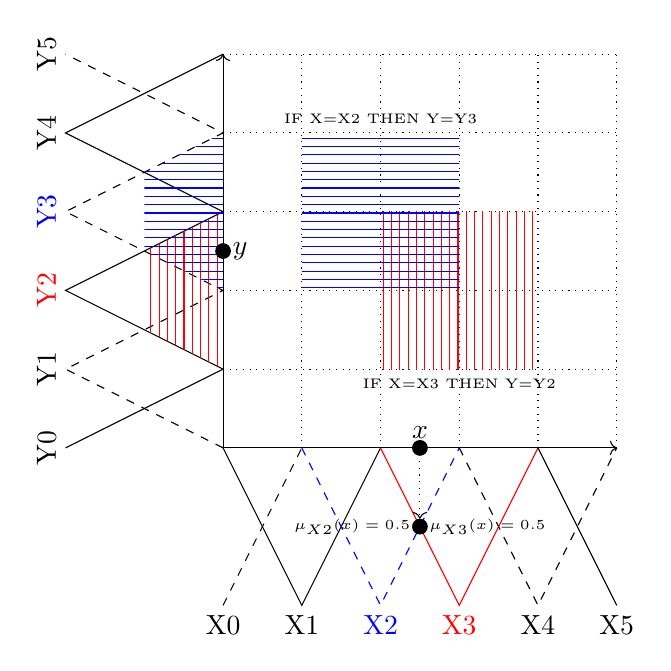
\begin{tikzpicture}

% eixos
\draw[<->] (0,5) -- (0,0) -- (5,0);

% triangulos horizontais
\draw (0,0) 
        -- (1,-2) node[below] {X1}
        -- (2,0) ;
\draw[red] (2,0) 
        -- (3,-2) node[red,below] {X3 }
        -- (4,0);
\draw   (4,0)
        -- (5,-2) node[below] {X5};

\draw[dashed] (0,-2) node[below] {X0}
        -- (1,0) ;
\draw[blue,dashed] (1,0)
        -- (2,-2) node[below,blue] {X2} 
        -- (3,0);
\draw[dashed] (3,0)
        -- (4,-2) node[below] {X4} 
        -- (5,0);

% triangulos verticais
\draw (-2,0) node[rotate=90,above] {Y0} 
        -- (0,1) 
        -- (-2,2) node[red,rotate=90,above] {Y2} 
        -- (0,3)
        -- (-2,4) node[rotate=90,above] {Y4} 
        -- (0,5);
\draw[dashed] (0,0) 
        -- (-2,1) node[rotate=90,above] {Y1} 
        -- (0,2) 
        -- (-2,3) node[blue,rotate=90,above] {Y3} 
        -- (0,4) 
        -- (-2,5) node[rotate=90,above] {Y5};

% retas verticais
\draw[dotted] (1,0) -- (1,5);
\draw[dotted] (2,0) -- (2,5);
\draw[dotted] (3,0) -- (3,5);
\draw[dotted] (4,0) -- (4,5);
\draw[dotted] (5,0) -- (5,5);

% retas horizontais
\draw[dotted] (0,1) -- (5,1);
\draw[dotted] (0,2) -- (5,2);
\draw[dotted] (0,3) -- (5,3);
\draw[dotted] (0,4) -- (5,4);
\draw[dotted] (0,5) -- (5,5);

\fill[black] (2.5,0) circle [radius=0.1] node[above] {$x$};
\draw[dotted,->] (2.5,0) -- (2.5,-0.9);
\fill[black] (2.5,-1) circle [radius=0.1] node[right,font=\tiny] {$\mu_{X3}(x)=0.5$};
\node[left,font=\tiny] at (2.5,-1) {$\mu_{X2}(x)=0.5$};

\fill[pattern color=red,pattern=vertical lines] (2,1) rectangle (4,3) ;
\fill[pattern color=blue,pattern=horizontal lines] (1,2) rectangle (3,4) ;

\node[font=\tiny] at (2,4) [above] {IF X=X2 THEN Y=Y3};
\node[font=\tiny] at (3,1) [below] {IF X=X3 THEN Y=Y2};

\fill[pattern color=red,pattern=vertical lines] (0,1) -- (-1,1.5) -- (-1,2.5) -- (0,3);
\fill[pattern color=blue,pattern=horizontal lines] (0,2) -- (-1,2.5) -- (-1,3.5) -- (0,4);

\fill[black] (0,2.5) circle [radius=0.1] node[right] {$y$};


\end{tikzpicture}
    \caption{Duas regras ativadas simultaneamente de um conjunto de regras, a partir de uma entrada $x$, são agregadas e uma função de defuzzificação, como o centróide, é usada para determinar $y$}
    \label{fig:2R}
\end{figure}

\begin{figure}
    \centering
    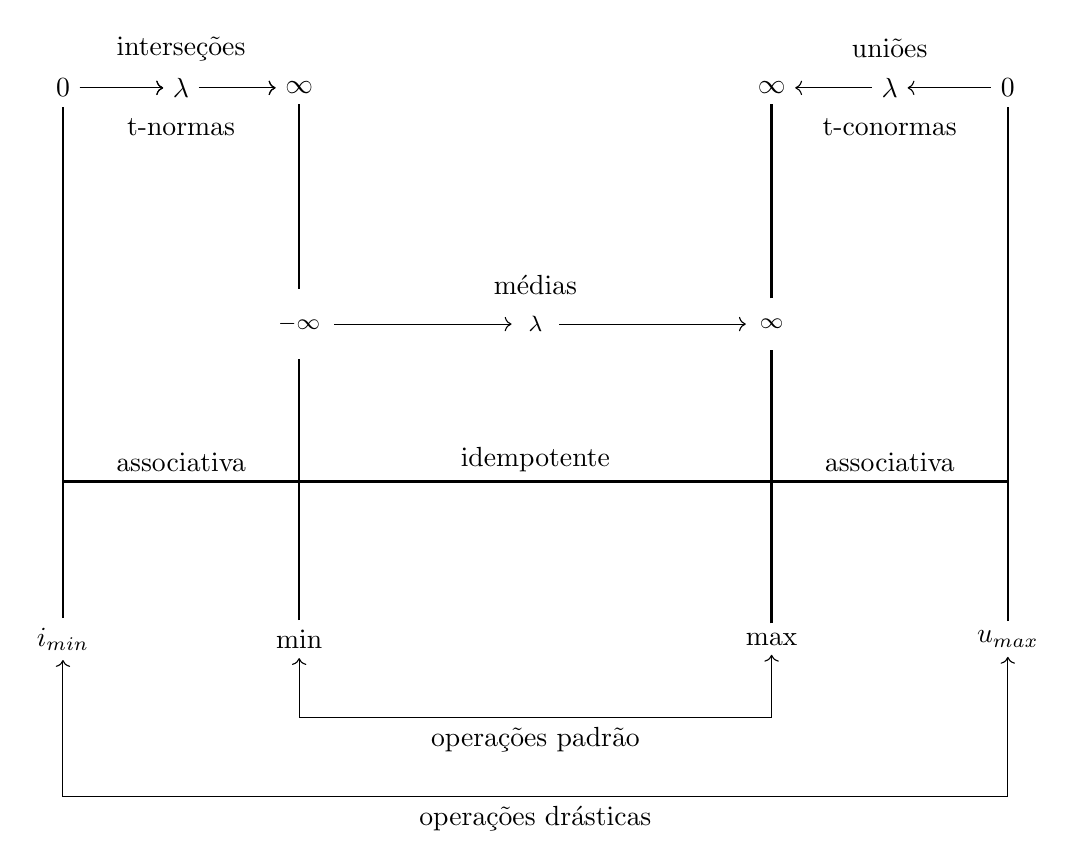
\begin{tikzpicture}
    [ bola/.style={circle,draw=white, fill=white,font=\footnotesize,text=black} ]
    
    \node (n1) at (0,10) {$0$} ;
    \node (n2) at (1.5,10) {$\lambda$};
    \node (n3) at (3,10) {$\infty$} ;  

    \draw[->] (n1.east) -- (n2.west);
    \draw[->] (n2.east) -- (n3.west);

    \node (n6) at (12,10) {$0$} ;
    \node (n5) at (10.5,10) {$\lambda$};
    \node (n4) at (9,10) {$\infty$} ;  
    
    \draw[<-] (n4.east) -- (n5.west);
    \draw[<-] (n5.east) -- (n6.west);
        
    \node (nimn) at  (0,3) {$i_{min}$};
    \node (numax) at (12,3) {$u_{max}$};
    \node (min) at (3,3) {$\min$};
    \node (max) at (9,3) {$\max$};
    \node at (1.5,10.5)  {interseções};
    \node at (1.5,9.5) {t-normas};
    \node at (10.5,10.5)  {uniões};
    \node at (10.5,9.5) {t-conormas};

    \draw[<->] (nimn.south) -- (0,1) -- (12,1)--(numax.south);
    \draw[<->] (min.south) -- (3,2) -- (9,2) --(max.south) ;

    \draw[->] (n1.east) -- (n2.west);
    \draw[->] (n2.east) -- (n3.west);


    \draw[thick] (0,5) -- (12,5);
    \node at (1.5,5) [above] {associativa};
    \node at (6,5) [above]   {idempotente};
    \node at (10.5,5) [above] {associativa};
    \node at (6,2) [below] {operações padrão};
    \node at (6,1) [below] {operações drásticas};
        
    \node (m1) at (3,7) [bola] {$-\infty$};
    \node (m2) at (6,7) [bola] {$\lambda$};
    \node (m3) at (9,7) [bola] {$\infty$};
    \draw[->] (m1.east) -- (m2.west);    
    \draw[->] (m2.east) -- (m3.west);    
    \node at (6,7.5) {médias};
    
    \draw[thick] (nimn.north) -- (n1.south);
    \draw[thick] (min.north) -- (m1.south) ;
    \draw[thick] (m1.north) -- (n3.south);
    \draw[thick] (max.north) -- (m3.south);
    \draw[thick] (m3.north) -- (n4.south);
    \draw[thick] (numax.north) -- (n6.south);

    \end{tikzpicture}
    \caption{Variáveis e posições}
    \label{fig:concepts1}
\end{figure}

\section{Modelo de Qualidade de Software}

Com exemplo, \ref{fig:qrocha}, de como trabalhar o posicionamento de forma relativa e com pontos pré-determinados via tikzmath.

\begin{figure}
    \centering
    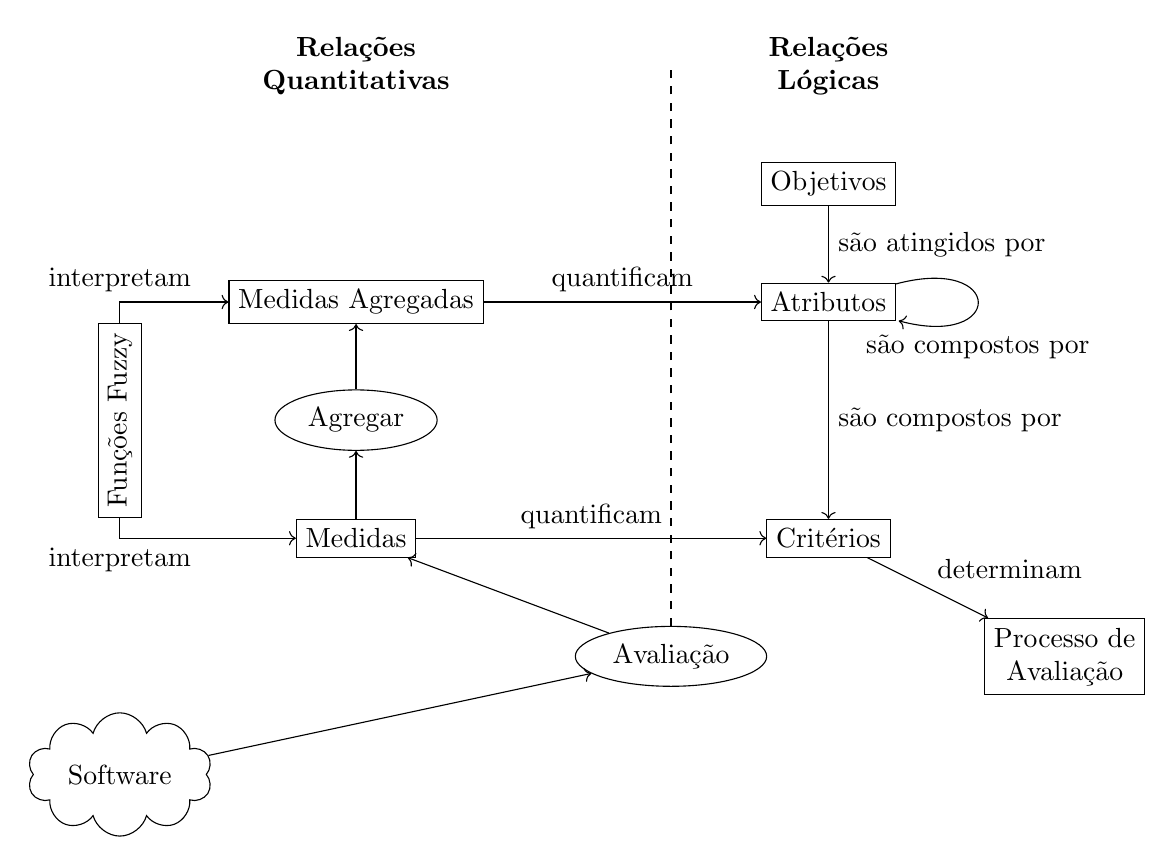
\begin{tikzpicture}
    \tikzmath{  \yd = 1.5 ; 
                \xd = 2 ;
                \x1 = 0 ; 
                \y1 = 0 ;
                \x2 = \x1 + \xd*1.5 ;
                \x3 = \x2 + 2*\xd ;
                \x4 = \x3 + \xd ;
                \x6 = \x4 + \xd ;
                \x5 = \x4 + 1.5*\xd ;
                \y2 = \y1 + \yd ;
                \y3 = \y2 + \yd ;
                \y4 = \y3 + \yd ;
                \y5 = \y4 + \yd ;
                \y6 = \y5 + \yd ;
                \y7 = \y6 + \yd ;         
                }
    \node[cloud,draw,aspect=2] (software) at (\x1,\y1) {Software};
    \node[ellipse,align=center,draw] (avaliacao) at (\x3,\y2) {Avaliação};
    \node[draw=black,rectangle] (medidas) at (\x2,\y3) {Medidas};
    \node[draw=black,rectangle] (crit) at (\x4,\y3) {Critérios};
    \node[rectangle,align=center,draw] (proc) at (\x5,\y2) {Processo de\\ Avaliação};
    \node[draw=black,ellipse,draw] (agre) at (\x2,\y4) {Agregar};
    \node[draw=black,rectangle] (medagre) at (\x2,\y5) {Medidas Agregadas};
    \node[draw=black,rectangle] (atrib) at (\x4,\y5)  {Atributos} edge [in=30,out=60,loop right] node[below=0.3]{são  compostos por} ();
    \node[draw=black,rectangle] (obj) at (\x4,\y6) {Objetivos};
    \node[align=center] (rq) at (\x2,\y7) {\textbf{Relações} \\  \textbf{Quantitativas}};
    \node[align=center] (rl) at (\x4,\y7) {\textbf{Relações} \\ \textbf{Lógicas}};
    \node[rectangle,draw,rotate=90] (fz) at (\x1,\y4) {Funções Fuzzy};
    
    \draw[thick,dashed] (avaliacao.north) -- (\x3,\y7) ;
    \draw[->] (software) -- (avaliacao);
    \draw[->] (avaliacao) -- (medidas);
    \draw[->] (medidas) -- (agre);
    \draw[->] (agre) -- (medagre);
    \draw[->] (medagre) -- node [midway,above] {quantificam} (atrib);
    \draw[->] (medidas) --node [midway,above] {quantificam}  (crit);
    \draw[->] (crit) -- node [midway, above right] {determinam} (proc);
    \draw[->] (atrib) --node [midway,right] {são compostos por}  (crit);
\draw[->] (obj) -- node [midway,right] {são atingidos por}  (atrib);
    
    \draw[->] (fz.east) |- node [midway,above] {interpretam} (medagre.west);
    \draw[->] (fz.west) |- node [midway,below] {interpretam} (medidas.west);
\end{tikzpicture} 
    \caption{Modelo Fuzzy de Qualidade Rocha }
    \label{fig:qrocha}
\end{figure}


\begin{figure}[h]
\centering

\begin{tikzpicture}
 \draw[decorate,decoration={coil, aspect=0}] (0,0) circle (1.5cm);
\end{tikzpicture}
    \caption{Decorations need many libraries (at least)}
    
\end{figure}

\begin{figure}
    \centering
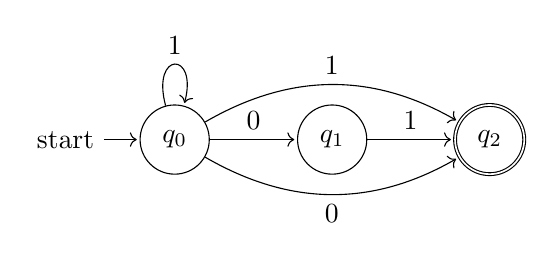
\begin{tikzpicture}[shorten >=1pt,node distance=2cm,on grid]
\node[state,initial] (q_0) {$q_0$};
\node[state] (q_1) [right=of q_0] {$q_1$};
\node[state,accepting](q_2) [right=of q_1] {$q_2$};
\path[->] (q_0) edge node [above] {0} (q_1)
edge [loop above] node {1} ()
edge [bend left] node [above] {1} (q_2)
edge [bend right] node [below] {0} (q_2)
(q_1) edge node [above] {1} (q_2);
\end{tikzpicture}
    \caption{Do manual topaths}
    
\end{figure}

\begin{figure}[h]
\centering
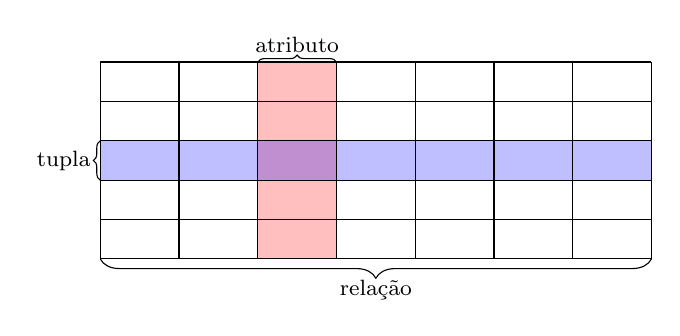
\begin{tikzpicture}
\fill[red,nearly transparent] (2,0) rectangle (3,2.5);
\fill[blue,nearly transparent] (0,1) rectangle (7,1.5);

\draw [decorate,decoration={brace}]
(2,2.5) -- (3,2.5)node [black,midway,above] {\footnotesize
 atributo };

\draw [decorate,decoration={brace}]
(0,1) -- (0,1.5)node [black,midway,left] {\footnotesize tupla};

\foreach \x in {0,1,2,3,4,5,6,7}
    \draw (\x,0) -- (\x,2.5);
\foreach \y in {0,.5,1,1.5,2,2.5}    
    \draw (0,\y) -- (7,\y);

\draw [decorate,decoration={brace,mirror,amplitude=7pt}]
(0,0) -- (7,0)node [black,midway,below=4pt] {\footnotesize{relação}};


\end{tikzpicture}


    \caption{Modelo abstrato de uma relação como uma tabela - usando decorations de chaves}
    \label{fig:reltab}
\end{figure}



\begin{figure}
\centering
\vspace*{350pt}
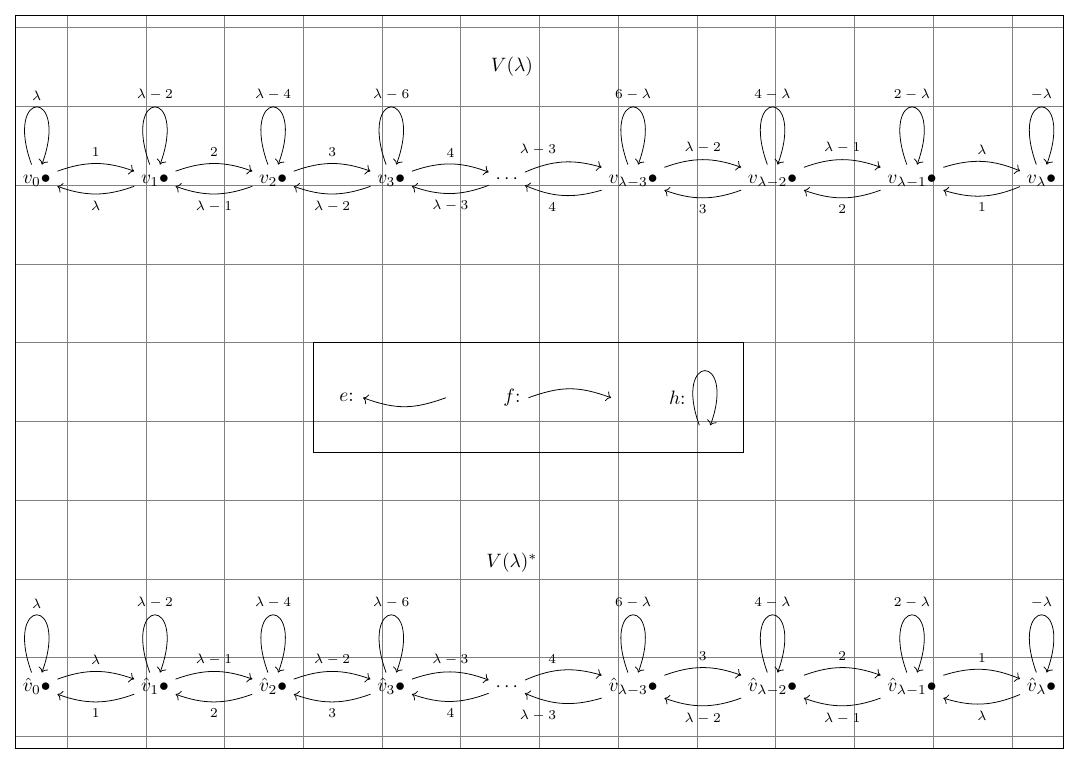
\begin{tikzpicture}[description/.style={fill=white,inner sep=2pt},show background grid,show background rectangle]
    \useasboundingbox (-6.5,-5) rectangle (6.5,4);
    \scope[transform canvas={scale=.7}]
      \matrix (m) [matrix of math nodes, row sep=31pt,
    column sep=40pt, text height=1.5ex, text depth=0.25ex]
    { \\ \\ \\ \underset{v_0}{\bullet} & \underset{v_1}{\bullet} & \underset{v_2}{\bullet} & \underset{v_3}{\bullet} & \cdots & \underset{v_{\lambda - 3}}{\bullet} & \underset{v_{\lambda - 2}}{\bullet} & \underset{v_{\lambda - 1}}{\bullet} & \underset{v_\lambda}{\bullet} \\ \\ \\ \\ \\ \\ \\ \\ \underset{\hat v_0}{\bullet} & \underset{\hat v_1}{\bullet} & \underset{\hat v_2}{\bullet} & \underset{\hat v_3}{\bullet} & \cdots & \underset{\hat v_{\lambda - 3}}{\bullet} & \underset{\hat v_{\lambda - 2}}{\bullet} & \underset{\hat v_{\lambda - 1}}{\bullet} & \underset{\hat v_\lambda}{\bullet} \\};
    \path[->,font=\scriptsize]
    (m-4-1) edge [bend left=20] node[auto] {$1$} (m-4-2)
    (m-4-2) edge [bend left=20] node[auto] {$\lambda$} (m-4-1)
            edge [bend left=20] node[auto] {$2$} (m-4-3)
    (m-4-3) edge [bend left=20] node[auto] {$\lambda - 1$} (m-4-2)
            edge [bend left=20] node[auto] {$3$} (m-4-4)
    (m-4-4) edge [bend left=20] node[auto] {$\lambda - 2$} (m-4-3)
            edge [bend left=20] node[auto] {$4$} (m-4-5)
    (m-4-5) edge [bend left=20] node[auto] {$\lambda - 3$} (m-4-4)
            edge [bend left=20] node[auto] {$\lambda - 3$} (m-4-6)
    (m-4-6) edge [bend left=20] node[auto] {$4$} (m-4-5)
            edge [bend left=20] node[auto] {$\lambda - 2$} (m-4-7)
    (m-4-7) edge [bend left=20] node[auto] {$3$} (m-4-6)
            edge [bend left=20] node[auto] {$\lambda - 1$} (m-4-8)
    (m-4-8) edge [bend left=20] node[auto] {$2$} (m-4-7)
            edge [bend left=20] node[auto] {$\lambda$} (m-4-9)
    (m-4-9) edge [bend left=20] node[auto] {$1$} (m-4-8);
    \draw[<-] (m-4-1) .. controls +(70:50pt) and +(110:50pt) .. node[pos=.5, above]{\scriptsize $\lambda$} (m-4-1);
    \draw[<-] (m-4-2) .. controls +(70:50pt) and +(110:50pt) .. node[pos=.5, above]{\scriptsize $\lambda - 2$} (m-4-2);
    \draw[<-] (m-4-3) .. controls +(70:50pt) and +(110:50pt) .. node[pos=.5, above]{\scriptsize $\lambda - 4$} (m-4-3);
    \draw[<-] (m-4-4) .. controls +(70:50pt) and +(110:50pt) .. node[pos=.5, above]{\scriptsize $\lambda - 6$} (m-4-4);
    \draw[<-] (m-4-6) .. controls +(70:50pt) and +(110:50pt) .. node[pos=.5, above]{\scriptsize $6 - \lambda$} (m-4-6);
    \draw[<-] (m-4-7) .. controls +(70:50pt) and +(110:50pt) .. node[pos=.5, above]{\scriptsize $4 - \lambda$} (m-4-7);
    \draw[<-] (m-4-8) .. controls +(70:50pt) and +(110:50pt) .. node[pos=.5, above]{\scriptsize $2 - \lambda$} (m-4-8);
    \draw[<-] (m-4-9) .. controls +(70:50pt) and +(110:50pt) .. node[pos=.5, above]{\scriptsize $-\lambda$} (m-4-9);
    \path[draw] (-4.1, -2) rectangle (3.7, 0);
    \draw (-3.5, -1) node {$e$:};
    \draw[<-] (-3.2, -1) .. controls +(-20:18pt) and +(200:18pt) .. (-1.7, -1);
    \draw (-.5, -1) node {$f$:};
    \draw[->] (-.2, -1) .. controls +(20:18pt) and +(160:18pt) .. (1.3, -1);
    \draw (2.5, -1) node {$h$:};
    \draw[<-] (3.1, -1.5) .. controls +(70:40pt) and +(110:40pt) ..  (2.9, -1.5);
    \draw (-.5, 5) node {$V(\lambda)$};
    \path[->,font=\scriptsize]
    (m-12-1) edge [bend left=20] node[auto] {$\lambda$} (m-12-2)
    (m-12-2) edge [bend left=20] node[auto] {$1$} (m-12-1)
            edge [bend left=20] node[auto] {$\lambda - 1$} (m-12-3)
    (m-12-3) edge [bend left=20] node[auto] {$2$} (m-12-2)
            edge [bend left=20] node[auto] {$\lambda - 2$} (m-12-4)
    (m-12-4) edge [bend left=20] node[auto] {$3$} (m-12-3)
            edge [bend left=20] node[auto] {$\lambda - 3$} (m-12-5)
    (m-12-5) edge [bend left=20] node[auto] {$4$} (m-12-4)
            edge [bend left=20] node[auto] {$4$} (m-12-6)
    (m-12-6) edge [bend left=20] node[auto] {$\lambda - 3$} (m-12-5)
            edge [bend left=20] node[auto] {$3$} (m-12-7)
    (m-12-7) edge [bend left=20] node[auto] {$\lambda - 2$} (m-12-6)
            edge [bend left=20] node[auto] {$2$} (m-12-8)
    (m-12-8) edge [bend left=20] node[auto] {$\lambda - 1$} (m-12-7)
            edge [bend left=20] node[auto] {$1$} (m-12-9)
    (m-12-9) edge [bend left=20] node[auto] {$\lambda$} (m-12-8);
    \draw[<-] (m-12-1) .. controls +(70:50pt) and +(110:50pt) .. node[pos=.5, above]{\scriptsize $\lambda$} (m-12-1);
    \draw[<-] (m-12-2) .. controls +(70:50pt) and +(110:50pt) .. node[pos=.5, above]{\scriptsize $\lambda - 2$} (m-12-2);
    \draw[<-] (m-12-3) .. controls +(70:50pt) and +(110:50pt) .. node[pos=.5, above]{\scriptsize $\lambda - 4$} (m-12-3);
    \draw[<-] (m-12-4) .. controls +(70:50pt) and +(110:50pt) .. node[pos=.5, above]{\scriptsize $\lambda - 6$} (m-12-4);
    \draw[<-] (m-12-6) .. controls +(70:50pt) and +(110:50pt) .. node[pos=.5, above]{\scriptsize $6 - \lambda$} (m-12-6);
    \draw[<-] (m-12-7) .. controls +(70:50pt) and +(110:50pt) .. node[pos=.5, above]{\scriptsize $4 - \lambda$} (m-12-7);
    \draw[<-] (m-12-8) .. controls +(70:50pt) and +(110:50pt) .. node[pos=.5, above]{\scriptsize $2 - \lambda$} (m-12-8);
    \draw[<-] (m-12-9) .. controls +(70:50pt) and +(110:50pt) .. node[pos=.5, above]{\scriptsize $-\lambda$} (m-12-9);
    \draw (-.5, -4) node {$V(\lambda)^\ast$};
    \endscope
\end{tikzpicture}
\caption{
The manual states: “Tracking of the picture size is (locally) switched off …”
This means that the bounding box is lost, which needs to be specified manually via the useasboundingbox path (= path[use as bounding box]) which also needs to be outside of the scope that has transform canvas applied to.
You might consider the necessarity to transform your whole picture (this also affects font-sizes!).
} \label{figV}
\end{figure}

\begin{figure}
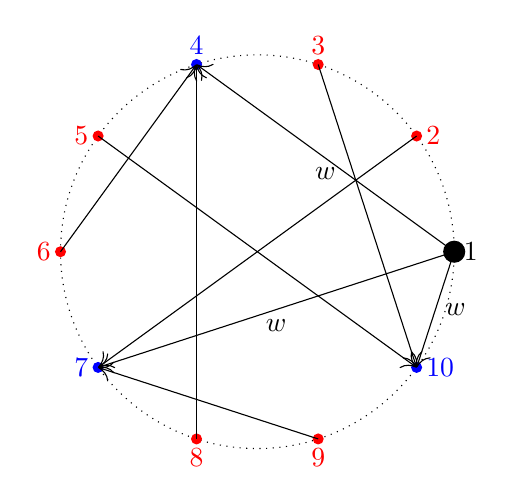
\begin{tikzpicture}
  \coordinate (center) at (1,2);
  \def\radius{2.5cm}
  % a circle
  \draw[dotted] (center) circle[radius=\radius];

  
  \fill[black] (center) ++(0:\radius)
  circle[radius=4pt] node[black,right] {1} ;
  
  \fill[red] (center) ++(36:\radius)
  circle[radius=2pt] node[right] {2};
  
  \fill[red] (center) ++(2*36:\radius)
  circle[radius=2pt] node[above] {3};
  
  \fill[blue] (center) ++(3*36:\radius)
  circle[radius=2pt] node[above] {4};
  
  \fill[red] (center) ++(4*36:\radius)
  circle[radius=2pt] node[left] {5};
  
  \fill[red] (center) ++(5*36:\radius)
  circle[radius=2pt] node[left] {6};
  
  \fill[blue] (center) ++(6*36:\radius)
  circle[radius=2pt] node[left] {7};
  
  \fill[red] (center) ++(7*36:\radius)
  circle[radius=2pt] node[below] {8};
  
  \fill[red] (center) ++(8*36:\radius)
  circle[radius=2pt] node[below] {9};
  
  \fill[blue] (center) ++(9*36:\radius)
  circle[radius=2pt] node[right] {10};
  
  
  \draw[-{>[scale=2.5,
          length=2,
          width=3]}]  (center)+(4*36:\radius) --   
          +(9*36:\radius) ;
   \draw[-{>[scale=2.5,
          length=2,
          width=3]}]  (center)+(2*36:\radius) --   
          +(9*36:\radius) ;
   \draw[-{>[scale=2.5,
          length=2,
          width=3]}]  (center)+(0:\radius) --   
          +(9*36:\radius) node [midway, right] {$w$};
 
   \draw[-{>[scale=2.5,
          length=2,
          width=3]}]  (center)+(7*36:\radius) --   
          +(3*36:\radius) ;
   \draw[-{>[scale=2.5,
          length=2,
          width=3]}]  (center)+(5*36:\radius) --   
          +(3*36:\radius) ;
   \draw[-{>[scale=2.5,
          length=2,
          width=3]}]  (center)+(0:\radius) --   
          +(3*36:\radius) node [midway, below] {$w$};
          
  \draw[-{>[scale=2.5,
          length=2,
          width=3]}]  (center)+(1*36:\radius) --   
          +(6*36:\radius) ;
   \draw[-{>[scale=2.5,
          length=2,
          width=3]}]  (center)+(8*36:\radius) --   
          +(6*36:\radius) ;
   \draw[-{>[scale=2.5,
          length=2,
          width=3]}]  (center)+(0:\radius) --   
          +(6*36:\radius) node [midway, below] {$w$};  
                 
\end{tikzpicture}
\caption{pontos em um círculo com cordas entre eles, exemplo de notação + e variação do tamanho da seta}
\end{figure}

\begin{figure}
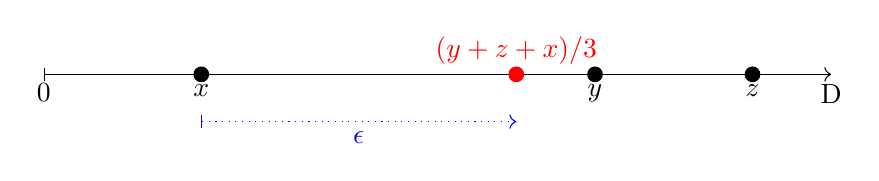
\begin{tikzpicture}
\draw[|->] node[below] {0}  (0,0) -- (10,0)node[below] {D};
\fill[black] (2,0) circle [radius=0.1] node[below] {$x$};
\fill[black] (7,0) circle [radius=0.1] node[below] {$y$};
\fill[black] (9,0) circle [radius=0.1] node[below] {$z$};
\draw[|->,blue,dotted] (2,-0.6) -- (4,-0.6) node[below] {$\epsilon$} -- (6,-0.6);
\fill[red] (6,0)  circle [radius=0.1] node[above] {$(y+z+x)/3$};
\end{tikzpicture}
\caption{Visão gráfica da medida simples de concordância para três pontos, x basicamente em desacordo, considerando um contra a média de todos}
    \label{fig:XYZ2}
\end{figure}

\begin{figure}
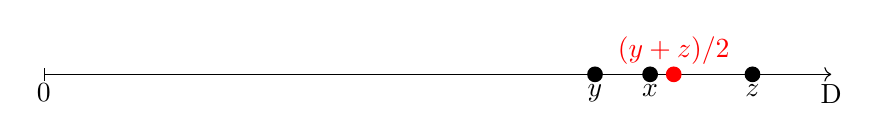
\begin{tikzpicture}
\draw[|->] node[below] {0}  (0,0) -- (10,0)node[below] {D};
\fill[black] (7.7,0) circle [radius=0.1] node[below] {$x$};
\fill[black] (7,0) circle [radius=0.1] node[below] {$y$};
\fill[black] (9,0) circle [radius=0.1] node[below] {$z$};
\fill[red] (8,0)  circle [radius=0.1] node[above] {$(y+z)/2$};
\end{tikzpicture}
\caption{Visão gráfica da medida simples de concordância para três pontos, x basicamente em acordo}
    \label{fig:PDF}
\end{figure}


\tikzset{
node of list/.style = { 
             draw, 
             fill=orange!20, 
             minimum height=6mm, 
             minimum width=6mm,
             node distance=6mm
   },
link/.style = {
     -stealth,
     shorten >=1pt
     },
array element/.style = {
    draw, fill=white,
    minimum width = 6mm,
    minimum height = 10mm
  }
}
\def\LinkedList#1{%
  \foreach \element in \list {
     \node[node of list, right = of aux, name=ele] {\element};
     \node[node of list, name=aux2, anchor=west] at ([xshift=-.4pt] ele.east) {};
     \draw[link] (aux) -- (ele);
     \coordinate (aux) at (aux2);
   }
   \fill (aux) circle(2pt);
}

\begin{figure}
\centering
\begin{tikzpicture}
\foreach \index/\list in {
.2/{(3,11),(16,24),null}, 
.4/{(4,10),(17,23),null}, 
.6/{(5,9),(18,22),null},
.8/{(6,8),(19,21),null},
1/{7,20,null}} {
   \node[array element] (aux) at (0,-\index*5) {\index};
   \LinkedList{\list}
}
\end{tikzpicture}
    \caption{Exemplo de uma lista de listas que serve como estrutura de dados baseada em cortes-$\alpha$ para o conjunto fuzzy ``perto de 7 ou 20''}
    \label{fig:alphacutlist}
\end{figure}

\begin{figure}
\centering

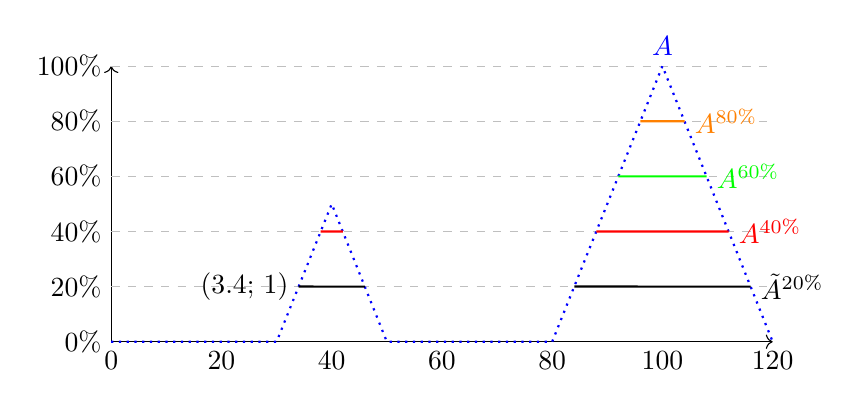
\begin{tikzpicture}[scale=0.7]

\def\pttocm#1{\pgfmathparse{#1 / 19.93333
    }\pgfmathprintnumber{\pgfmathresult}}
    
    \newcommand{\printcoords}[1]{
      \newdimen\posx
      \pgfextractx{\posx}{\pgfpointanchor{#1}{center}}
      \newdimen\posy
      \pgfextracty{\posy}{\pgfpointanchor{#1}{center}}
      (\pttocm\posx ; \pttocm\posy )
    }
    
    
\draw[<->] (0,5) -- (0,0) -- (12,0);
\node[left] at (0,5) {$100\%$};
\node[left] at (0,4) {$80\%$};
\node[left] at (0,3) {$60\%$};
\node[left] at (0,2) {$40\%$};
\node[left] at (0,1) {$20\%$};
\node[left] at (0,0) {$0\%$};
\draw[style=dashed,color=gray!50] (0,5) -- (12,5);
\draw[style=dashed,color=gray!50] (0,4) -- (12,4);
\draw[style=dashed,color=gray!50] (0,3) -- (12,3);
\draw[style=dashed,color=gray!50] (0,2) -- (12,2);
\draw[style=dashed,color=gray!50] (0,1) -- (12,1);
\node[below] at (12,0) {$120$};
\node[below] at (10,0) {$100$};
\node[below] at (8,0) {$80$};
\node[below] at (6,0) {$60$};
\node[below] at (4,0) {$40$};
\node[below] at (2,0) {$20$};
\node[below] at (0,0) {$0$};
\draw[color=blue,style=thick,style=dotted,name path=vava] (0,0) -- (3,0) -- (4,2.5) -- (5,0) -- (8,0)-- (10,5) node[above] {$\Tilde{A}$} -- (12,0);
\path[name path=xixi,draw=none] (0,1) -- (12,1);
\path[name intersections={of=vava and xixi }];
\coordinate (A) at (intersection-1);
\coordinate (B) at (intersection-2);
\coordinate (C) at (intersection-3);
\coordinate (D) at (intersection-4);
\draw[color=black,style=thick] (A) node[left] {\printcoords{A}} -- (B);
\draw[color=black,style=thick] (C) --  (D) node[right] {$\tilde{A}^{20\%}$}  ;
\path[name path=xuxu,draw=none] (0,2) -- (12,2);
\path[name intersections={of=vava and xuxu }];
\coordinate (A) at (intersection-1);
\coordinate (B) at (intersection-2);
\coordinate (C) at (intersection-3);
\coordinate (D) at (intersection-4);
\draw[color=red,style=thick] (A) -- (B);
\draw[color=red,style=thick] (C) -- (D) node[right] {$\Tilde{A}^{40\%}$};
\path[name path=xexe,draw=none] (0,3) -- (12,3);
\path[name intersections={of=vava and xexe }];
\coordinate (A) at (intersection-1);
\coordinate (B) at (intersection-2);
\draw[color=green,style=thick] (A) -- (B) node[right] {$\Tilde{A}^{60\%}$};
\path[name path=xaxa,draw=none] (0,4) -- (12,4);
\path[name intersections={of=vava and xaxa }];
\coordinate (A) at (intersection-1);
\coordinate (B) at (intersection-2);
\draw[color=orange,style=thick] (A) -- (B)node[right] {$\Tilde{A}^{80\%}$};
\end{tikzpicture}
    \caption{Exemplo de cortes-$\alpha$, onde as linhas horizontais indicam os valores do eixo das abcissas que pertencem ao conjunto nítido correspondente}
    \label{fig:medioalpha}
\end{figure}

\begin{figure}
    \centering
    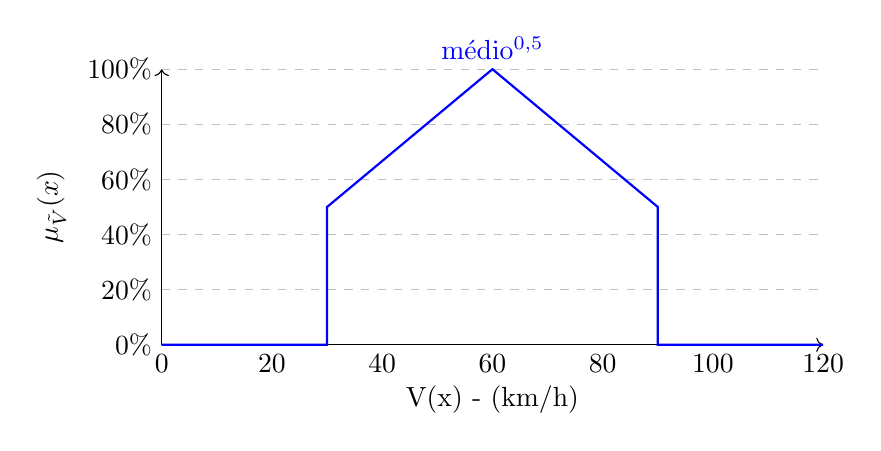
\begin{tikzpicture}[scale=0.7]
\draw[<->] (0,5) -- (0,0) -- (12,0);
\node[left] at (0,5) {$100\%$};
\node[left] at (0,4) {$80\%$};
\node[left] at (0,3) {$60\%$};
\node[left] at (0,2) {$40\%$};
\node[left] at (0,1) {$20\%$};
\node[left] at (0,0) {$0\%$};
\draw[style=dashed,color=gray!50] (0,5) -- (12,5);
\draw[style=dashed,color=gray!50] (0,4) -- (12,4);
\draw[style=dashed,color=gray!50] (0,3) -- (12,3);
\draw[style=dashed,color=gray!50] (0,2) -- (12,2);
\draw[style=dashed,color=gray!50] (0,1) -- (12,1);
\node[below] at (12,0) {$120$};
\node[below] at (10,0) {$100$};
\node[below] at (8,0) {$80$};
\node[below] at (6,0) {$60$};
\node[below] at (4,0) {$40$};
\node[below] at (2,0) {$20$};
\node[below] at (0,0) {$0$};
\draw[color=blue,style=thick] (0,0) -- (3,0) -- (3,2.5) -- (6,5) -- (9,2.5)-- (9,0) -- (12,0);
\node[rotate=90] at (-2,2.5) {$\mu_{\tilde{V}}(x)$};
\node at (6,-1) {V(x) - (km/h)};
\node[above,color=blue]  at (6,5) {médio$^{0,5}$};
\end{tikzpicture}
    \caption{O conjunto referente ao corte-alfa de médio com $\alpha=0,5$, ou seja médio$^{0,5}$.}
    \label{fig:medioalpha}
\end{figure}




\begin{figure}
    \centering
    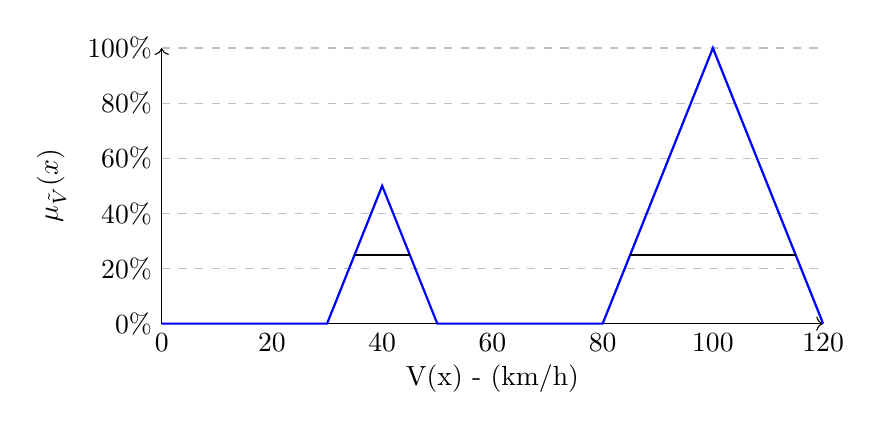
\begin{tikzpicture}[scale=0.7]
\draw[<->] (0,5) -- (0,0) -- (12,0);
\node[left] at (0,5) {$100\%$};
\node[left] at (0,4) {$80\%$};
\node[left] at (0,3) {$60\%$};
\node[left] at (0,2) {$40\%$};
\node[left] at (0,1) {$20\%$};
\node[left] at (0,0) {$0\%$};
\draw[style=dashed,color=gray!50] (0,5) -- (12,5);
\draw[style=dashed,color=gray!50] (0,4) -- (12,4);
\draw[style=dashed,color=gray!50] (0,3) -- (12,3);
\draw[style=dashed,color=gray!50] (0,2) -- (12,2);
\draw[style=dashed,color=gray!50] (0,1) -- (12,1);
\node[below] at (12,0) {$120$};
\node[below] at (10,0) {$100$};
\node[below] at (8,0) {$80$};
\node[below] at (6,0) {$60$};
\node[below] at (4,0) {$40$};
\node[below] at (2,0) {$20$};
\node[below] at (0,0) {$0$};
\node[rotate=90] at (-2,2.5) {$\mu_{\tilde{V}}(x)$};
\node at (6,-1) {V(x) - (km/h)};
\draw[color=blue,style=thick] (0,0) -- (3,0) -- (4,2.5) -- (5,0) -- (8,0)-- (10,5) -- (12,0);
\draw[color=black,style=thick] (3.5,1.25) -- (4.5,1.25);
\draw[color=black,style=thick] (8.5,1.25) -- (11.5,1.25);
\end{tikzpicture}
    \caption{Exemplo de cortes-$\alpha$}
    \label{fig:medioalpha}
\end{figure}

\begin{figure}
    \centering
    \begin{tikzpicture}[yscale=0.05,xscale=.3]
\draw[<->] (0,100) -- (0,0) -- (30,0);
\node[left] at (0,100) {$100\%$};
\node[left] at (0,80) {$80\%$};
\node[left] at (0,60) {$60\%$};
\node[left] at (0,40) {$40\%$};
\node[left] at (0,20) {$20\%$};
\node[left] at (0,0) {$0\%$};
\draw[style=dashed,color=gray!50] (0,100) -- (30,100);
\draw[style=dashed,color=gray!50] (0,80) -- (30,80);
\draw[style=dashed,color=gray!50] (0,60) -- (30,60);
\draw[style=dashed,color=gray!50] (0,40) -- (30,40);
\draw[style=dashed,color=gray!50] (0,20) -- (30,20);
\node[below] at (30,0) {$30$};
\node[below] at (25,0) {$25$};
\node[below] at (20,0) {$20$};
\node[below] at (15,0) {$15$};
\node[below] at (10,0) {$10$};
\node[below] at (5,0) {$5$};
\node[below] at (0,0) {$0$};

\draw[color=black,style=thick] (3,20) -- (11,20);
\draw[color=black,style=thick] (16,20) -- (24,20);

\draw[color=black,style=thick] (4,40) -- (10,40);
\draw[color=black,style=thick] (17,40) -- (23,40);

\draw[color=black,style=thick] (5,60) -- (9,60);
\draw[color=black,style=thick] (18,60) -- (22,60);

\draw[color=black,style=thick] (6,80) -- (8,80);
\draw[color=black,style=thick] (19,80) -- (21,80);

\node[rotate=90] at (-5,50) {$\mu_{\tilde{A}}(x)$};

\node at (15,-15) {x};

\end{tikzpicture}
    \caption{Representação dos cortes-$\alpha$ do conjunto $\tilde{A}$ dos números perto de 7 ou 20}
    \label{fig:repalpcut}
\end{figure}

\begin{figure}
    \centering
    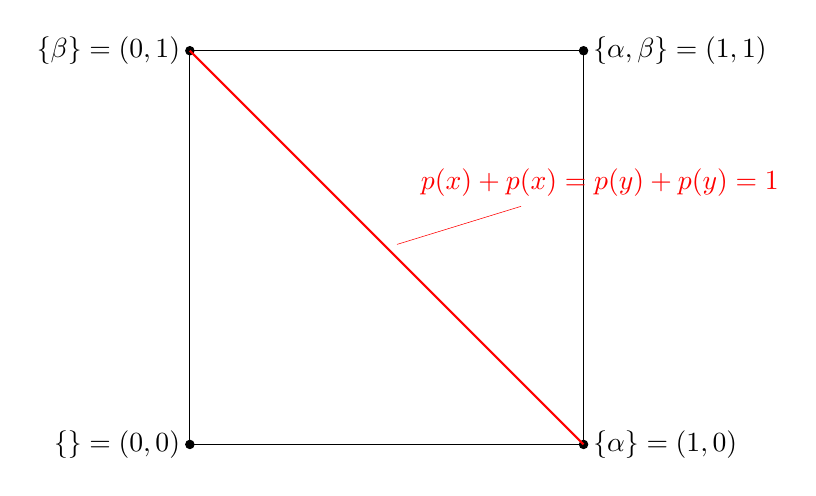
\begin{tikzpicture}
\draw  (0,0)-- (0,5) -- (5,5) -- (5,0) -- (0,0);
\draw[fill=black]  (0,0) circle (1.5pt);
\draw[fill=black]  (5,0) circle (1.5pt);
\draw[fill=black]  (0,5) circle (1.5pt);
\draw[fill=black]  (5,5) circle (1.5pt);
\node[left] at (0,0) {$\{\}=(0,0)$ };
\node[left] at (0,5) {$\{\beta\}=(0,1)$ };
\node[right] at (5,0) {$\{\alpha\}=(1,0)$};
\node[right] at (5,5) {$\{\alpha,\beta\}= (1,1)$};
\draw[color=red,style=thick] (0,5) -- (5,0) node [pin={[pin edge={solid,red}]60:{$p(x)+p(\Bar{x})=p(y)+p(\Bar{y})=1$}},midway] {};

\end{tikzpicture}
    \caption{Distribuições de probablidade só podem estar na reta onde a soma da probabilidade de pertencer ao conjunto e não pertencer ao conjunto é $1$ \cite{klir1995fuzzy} }
    \label{fig:3fuz}
\end{figure}

\begin{figure}[h]
\centering
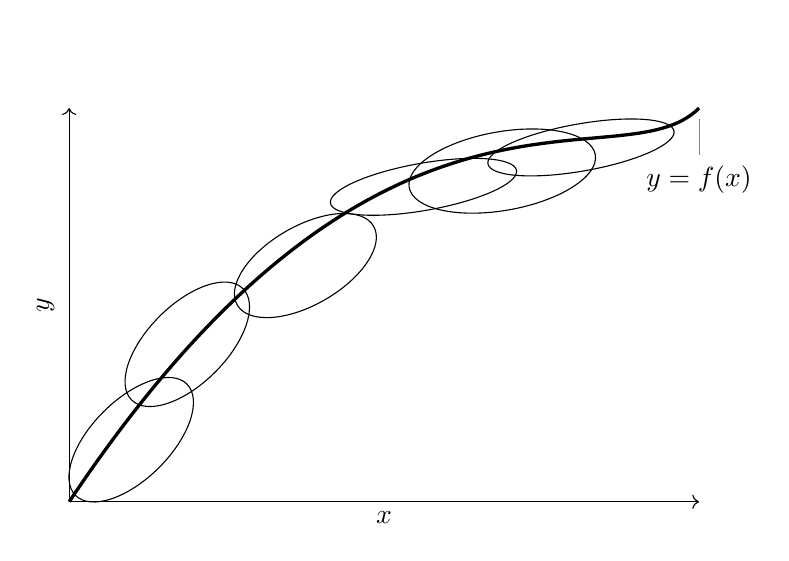
\begin{tikzpicture}
\draw[<->] (0,5) -- (0,0) -- (8,0);
\node[rotate=90] at (-.3,2.5) {$y$};
\node[below] at (4,0) {$x$};

\draw[very thick] (0,0) .. controls (4,6) and (7,4).. (8,5) node[pin=below:{$y=f(x)$}] { } ;
\draw[rotate around={45:(1,1)}] (0.7,1)ellipse [x radius=1, y radius=0.5];
\draw[rotate around={45:(1.5,2)}] (1.5,2)ellipse [x radius=1, y radius=0.5];
\draw[rotate around={30:(3,3)}] (3,3)ellipse [x radius=1, y radius=0.5];
\draw[rotate around={10:(4.5,4)}] (4.5,4)ellipse [x radius=1.2, y radius=0.3];
\draw[rotate around={10:(5.5,4.2)}] (5.5,4.2)ellipse [x radius=1.2, y radius=0.5];
\draw[rotate around={10:(6.5,4.5)}] (6.5,4.5)ellipse [x radius=1.2, y radius=0.3];
 \end{tikzpicture}
\end{figure}

\documentclass{article}
\usepackage[utf8]{inputenc}
\usepackage[T1]{fontenc}
\usepackage{lmodern}
% para usar "exatamente aqui" H opção em figure
\usepackage{float} 
\usepackage{makeidx} 
%%%%%%%%%%%%%%%%%%%%%%%%%%%%%%%%%%%%%%%%%%%%%%%%%%%%%%%%%
% Source: http://en.wikibooks.org/wiki/LaTeX/Hyperlinks %
%%%%%%%%%%%%%%%%%%%%%%%%%%%%%%%%%%%%%%%%%%%%%%%%%%%%%%%%%
\usepackage{hyperref}
\usepackage{graphicx}
\usepackage[utf8]{inputenc}
\usepackage[portuguese]{babel}
%\usepackage[english]{babel}

% for tkiz
\usepackage{pgf,tikz}
\usepackage{mathrsfs}
\usetikzlibrary{arrows}
\usetikzlibrary{arrows.meta}
\usetikzlibrary{mindmap} 
\usetikzlibrary{datavisualization}
\usetikzlibrary{datavisualization.formats.functions}
\usetikzlibrary{shapes.misc}
\usetikzlibrary{calc}
\usetikzlibrary{math}
\usetikzlibrary{shapes.symbols}
\usetikzlibrary{shapes.geometric}
\usetikzlibrary{patterns} 
\usetikzlibrary{positioning}  % distancia nos below
\usetikzlibrary{topaths} % loop edge
\usetikzlibrary{decorations} 
\usetikzlibrary{decorations.shapes}
\usetikzlibrary{decorations.pathmorphing}
\usetikzlibrary{decorations.text}
\usepgflibrary{decorations.pathreplacing} \usepgflibrary{decorations.markings} 
\usepgflibrary{decorations.footprints} 
\usepgflibrary{decorations.fractals} 
\usetikzlibrary{matrix} 
\usetikzlibrary{intersections} 



%
%
% Pacotes Xexéo
%
%
\usepackage{amsmath}
\usepackage{amsthm}
\usepackage{amssymb}
\usepackage{mdframed} % framed modules
\usepackage{listings} % listagns de programas
\newtheorem{theorem}{Teorema} 
%%%%%%%%%%%%%%%%%%%%%%%%%%
% definições

\newcommand{\NN}{\mathbb{N}}              % Natural numbers
\newcommand{\QQ}{\mathbb{Q}}              % Rationals
\newcommand{\RR}{\mathbb{R}}              % Reals
\newcommand{\ZZ}{\mathbb{Z}}              % Integers
%\newcommand{\powerset}{\mathcal{P}}       % power set
\newcommand{\setcomp}[1]{\overline{#1}}   % set complement
\newcommand{\negate}{{\sim}}              % negation (logic)
\newcommand{\xor}{\oplus}                 % xor
\renewcommand{\implies}{\Rightarrow}      % shorter version of =>
\renewcommand{\iff}{\Leftrightarrow}      % shorter <=>
\newcommand{\powerset}{\raisebox{.15\baselineskip}{\Large\ensuremath{\wp}}}

%%%%%%%%%%%%%%%%%%%%%
%%%%%%%%%%%%%%%%%%%%%
%%%%%%%%%%%%%%%%%%%%% ACENTOS EM LSTLISTING
%%%%%%%%%%%%%%%%%%%%% 
%%%%%%%%%%%%%%%%%%%%%
\lstset{language=Python,extendedchars=true,basicstyle=\ttfamily,inputencoding=utf8,
            literate=%
            {ã}{{\~{a}}}1
            {á}{{\'{a}}}1
            {â}{{\^{a}}}1
            {à}{{\`{a}}}1
            {é}{{\'{e}}}1
            {è}{{\`{e}}}1
            {ê}{{\^{e}}}1
            {î}{{\^{i}}}1
            {í}{{\'{i}}}1
            {ô}{{\^{o}}}1
            {ó}{{\'{o}}}1
            {õ}{{\~{o}}}1
            {û}{{\^{u}}}1
            {ú}{{\'{u}}}1
            {ç}{{\c{c}}}1
            {Ç}{{\c{C}}}1
            {Ã}{{\~{A}}}1
            {À}{{\`{A}}}1
            {Â}{{\^{A}}}1
            {Á}{{\'{A}}}1
            {É}{{\'{E}}}1
            {Ê}{{\^{E}}}1
            {Î}{{\^{I}}}1
            {Í}{{\'{I}}}1
            {Ó}{{\'{O}}}1
            {Ô}{{\^{O}}}1
            {Õ}{{\~{O}}}1
            {Ú}{{\'{U}}}1
            }


% no figures after footnote
\usepackage[bottom]{footmisc}

%%%%%%%%%%%%%%%
\renewcommand{\lstlistingname}{Programa}% Listing -> Algorithm
\renewcommand{\lstlistlistingname}{Lista de \lstlistingname s}% List of Listings -> List of Algorithms
% Define Language
\lstdefinelanguage{IEC61131}
{
  % list of keywords
  keywords={
    FUNCTION_BLOCK,
    VAR_INPUT,
    REAL,
    END_VAR,
    VAR_OUTPUT,
    FUZZIFY,
    TERM,
    END_FUZZIFY,
    DEFUZZIFY,
    METHOD:,
    END_DEFUZZIFY,
    RULEBLOCK,
    AND, MIN, ACT, MAX, ACCU, IS,
    ACCUM,
    RULE,
    IF, END,
    THEN,
    END_RULEBLOCK,
    END_FUNCTION_BLOCK
  },
  sensitive=true, % keywords are  case-sensitive
  columns=flexible,
  morecomment=[l]{//}, % l is for line comment
  morecomment=[s]{/*}{*/}, % s is for start and end delimiter
  morestring=[b]" % defines that strings are enclosed in double quotes,
  basicstyle=\scriptsize,
    numbers=left, % show line numbers at the left
  numberstyle=\tiny\ttfamily % style of the line numbers
}

\lstdefinelanguage{CLOUDSL}
{
  % list of keywords
  keywords={
  DATA,
  TYPE,
  VARINT,
  IN,
  AS,
  AUTOMATIC,
  VARSOLREAL,
  TERM,
  ALPHA,
  CURVE,
  TRIANGULAR,
  CONCENTRATOR,
  FACTOR,
  HEDGE,
  RULE,
  IF,
  AND,
  THEN,
  MODULE,
  EVALUATION,
  OUTPUT,
  TO,
  UNDECIDED,
  UNDEFINED,
  NULL,
  NOINFO,
  DILATION,
  SELECT,
  FROM,
  TO,
  WHERE,
  WITH,
  INTESIFICATION,
  BEGIN,
  END,
  LOADMODEL,
  BEGINMODEL,
  ENDMODEL,
  CREATE,
  TABLE
  FROM,
  ARQTEXT,
  ODBC,
  GIS,
  LINGTERM,
  GAUSS,
  TRAPEZ,
  CUSTOM
  CRISPVAR,
  LIGVAR,
  FUZZYVAR,
  FZYNUMBER,
  DOMAIN,
  OVER,
  OR,
  NOT,
  IS,
  EXECMODEL,
  EXEQUERY
  },
  sensitive=true, % keywords are  case-sensitive
  columns=flexible,
  morecomment=[l]{//}, % l is for line comment
  morecomment=[s]{/*}{*/}, % s is for start and end delimiter
  morestring=[b]" % defines that strings are enclosed in double quotes,
  basicstyle=\small\ttfamily,
    numbers=left, % show line numbers at the left
  numberstyle=\tiny\ttfamily % style of the line numbers
}

%%%%%%%%%%%%%%%%%%%%%%%%%%%%%%%%%%%%%%%%%%%%%%%%%%%
% First page of book which contains 'stuff' like: %
%  - Book title, subtitle                         %
%  - Book author name                             %
%%%%%%%%%%%%%%%%%%%%%%%%%%%%%%%%%%%%%%%%%%%%%%%%%%%



\title{Testes}
\author{Geraldo Xexéo}
\date{July 2017}

\usepackage[utf8]{inputenc}

\usepackage{pythontex}
\begin{document}
 



\begin{figure}[h]
\centering
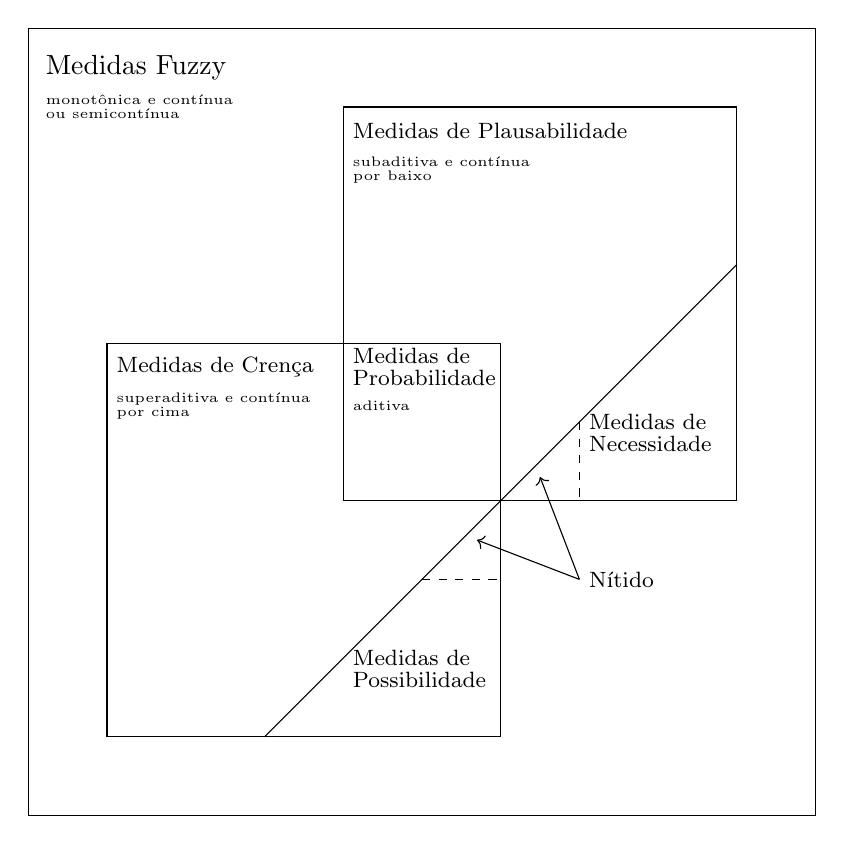
\begin{tikzpicture}

\draw  (0,0) rectangle (10,10) ;
\draw  (1,1) rectangle (6,6);
\draw  (4,4) rectangle (9,9);
\draw (3,1) -- (9,7) ;

\draw[dashed] (5,3) -- (6,3) ;
\draw[dashed] (7,5) -- (7,4) ;

\node at (0.1,9.5) [right] {Medidas Fuzzy};
\node at (0.1,9) [right,align=left,font=\fontsize{5pt}{5pt}\selectfont]
{monotônica e contínua \\ ou semicontínua};

\node at (4,5.7) [right,align=left,font=\fontsize{8pt}{8pt}\selectfont] 
{ Medidas de \\ Probabilidade};
\node at (4,5.2) [right,align=left,font=\fontsize{5pt}{5pt}\selectfont]
{aditiva};

\node at (1,5.7)
[right,align=left,font=\fontsize{8pt}{8pt}\selectfont] 
{Medidas de Crença};
\node at (1,5.2)
[right,align=left,font=\fontsize{5pt}{5pt}\selectfont]
{superaditiva e contínua \\ por cima };


\node at (4,8.7)
[right,align=left,font=\fontsize{8pt}{8pt}\selectfont]  
{Medidas de Plausabilidade};
\node at (4,8.2)
[right,align=left,font=\fontsize{5pt}{5pt}\selectfont]
{subaditiva e contínua \\ por baixo };

\node at (7,4.5)
[above right,align=left,font=\fontsize{8pt}{8pt}\selectfont]  
{Medidas de \\ Necessidade};

\node at (4,1.5)
[above right,align=left,font=\fontsize{8pt}{8pt}\selectfont]  
{Medidas de \\ Possibilidade};

\node at (7,3)
[right,align=left,font=\fontsize{8pt}{8pt}\selectfont] 
{Nítido};

\draw[->] (7,3) -- (6.5,4.3);
\draw[->] (7,3) -- (5.7,3.5);




\end{tikzpicture}


    \caption{Klir e os tipos de medida}
\end{figure}







\end{document}


\end{document}


